\documentclass{rvcepaper}
% s7-common.tex -- macros shared by the Sem 7 CIE papers (\input right after \documentclass{rvcepaper})
% placeholder for text that cannot be read in the scan
\newcommand{\illeg}{\textit{[illegible]}}
\newcommand{\illegc}{{\tiny\textit{[illegible]}}}
% question table with a custom header row: \begin{gtable}[PART -- A]{Sl.\newline No.}{Questions}{M}{BT}{CO}
% the optional title is set as the table's first row so it never strands at a page foot
\newcommand{\gtitlerow}{}
\newenvironment{gtable}[6][]{%
  \def\gtitle{#1}\ifx\gtitle\empty\def\gtitlerow{}\else\def\gtitlerow{\multicolumn{5}{c}{\bfseries\gtitle}\\*[2pt]}\fi
  \begin{longtable}{|C{1.05cm}|p{12.2cm}|C{0.95cm}|C{0.95cm}|C{0.95cm}|}
  \gtitlerow
  \hline \textbf{#2} & \multicolumn{1}{c|}{\textbf{#3}} & \textbf{#4} & \textbf{#5} & \textbf{#6}\\* \hline
  \endfirsthead
  \endhead
}{\end{longtable}}
\newcommand{\twonotes}[2]{{\small Note:}\par\vspace{-1pt}
\hspace*{0.5cm}{\footnotesize 1. \hspace{0.1cm}#1}\par
\hspace*{0.5cm}{\footnotesize 2. \hspace{0.1cm}#2}\par\vspace{3pt}}
\newcommand{\onenote}[1]{{\small Note:}\par\vspace{-1pt}
\hspace*{0.5cm}{\footnotesize 1. \hspace{0.1cm}#1}\par\vspace{3pt}}
% keep the BT/CO caption and the marks-distribution table on the same page
\renewcommand{\btfoot}[2]{\par\vspace{8pt}\noindent\begin{minipage}{\textwidth}\centering
  {\small BT-Blooms Taxonomy, CO-Course Outcomes, M-Marks}\par\vspace{2pt}
  \begin{tabular}{#1}#2\end{tabular}\end{minipage}\par\nopagebreak\vspace{2pt}}
\newcommand{\xfoot}[3]{\par\vspace{8pt}\noindent\begin{minipage}{\textwidth}\centering
  {\small #1}\par\vspace{2pt}\begin{tabular}{#2}#3\end{tabular}\end{minipage}\par\nopagebreak\vspace{2pt}}
\newcommand{\qq}[5]{#1 & #2 & #3 & #4 & #5\\}
\newcommand{\qm}[3]{#1 & #2 & #3\\ \hline}
% other-department header table (Date / Course Code / Sem rows + title row)
\newcommand{\ofour}[7]{\noindent\begingroup\renewcommand{\arraystretch}{1.3}\fontsize{11.5}{13}\selectfont
\begin{tabular}{|C{3.6cm}|C{4.6cm}|C{4.0cm}|C{3.8cm}|}\hline
Date & #1 & Maximum Marks & #2\\\hline
Course Code & #3 & Duration & #4\\\hline
Sem & #5 & \multicolumn{2}{c|}{#6}\\\hline
\multicolumn{4}{|c|}{\bfseries\fontsize{13}{15}\selectfont #7}\\\hline
\end{tabular}\endgroup\par\vspace{6pt}}
\renewcommand{\arraystretch}{1.05}
% the closing stars line stays with the block above it
\renewcommand{\stars}[1]{\par\nopagebreak\vspace{2pt}\nopagebreak\centerline{#1}}
% printed value struck through by hand, with the handwritten correction under it: \corr{60}{34}
\usepackage[normalem]{ulem}
\newcommand{\corr}[2]{\shortstack{\sout{#1}\\#2}}
\usetikzlibrary{decorations.pathmorphing}
% "Academic year" header table without the DEPARTMENT OF block (use inside iempaperB after \paperinfo)
\newcommand{\iemtableB}{%
  \par\vspace{4pt}\noindent\begingroup\renewcommand{\arraystretch}{1.5}\bfseries\fontsize{11.5}{13}\selectfont
  \begin{tabular}{|p{4.2cm}|p{5.0cm}|p{3.7cm}|p{3.6cm}|}\hline
   Date & \getkey{date} & Maximum Marks & \getkey{maxmarks}\\\hline
   Course Code & \getkey{code} & Duration & \getkey{duration}\\\hline
   Sem & \getkey{sem} & \multicolumn{2}{l|}{\getkey{exam}}\\\hline
   \multicolumn{4}{|c|}{\getkey{title}}\\\hline
  \end{tabular}\endgroup\par\vspace{4pt}}
% other-department CIE header: \xdept{Department line}{left1}{mid1}{right1}{left2}{mid2}{right2}{course title cell}{right3}
\newcommand{\xdept}[9]{\par\vspace{2pt}\centerline{\bfseries\fontsize{13.5}{16}\selectfont #1}\par\vspace{4pt}
  \noindent\begingroup\renewcommand{\arraystretch}{1.5}\bfseries\fontsize{11.5}{13}\selectfont
  \begin{tabular}{|p{4.8cm}|C{5.6cm}|p{5.7cm}|}\hline
  #2 & #3 & #4\\\hline #5 & #6 & #7\\\hline \multicolumn{2}{|p{10.8cm}|}{#8} & #9\\\hline
  \end{tabular}\endgroup\par\vspace{8pt}}

\begin{document}

% ---------- HS271TA Indian Knowledge System
\begin{iempaperB}
\paperinfo{ayear={2025-2026 (Odd Semester)},usn=0,date={Dec 2025},code={HS271TA},sem={VII},exam={\hfill CIE II\hfill\mbox{}},maxmarks={50 + 10},duration={120 Min},
 title={INDIAN KNOWLEDGE SYSTEM},shownote=0}
\iemtableB
\begin{gtable}[{\hfill PART -- A\hfill\llap{\normalfont(10 Marks)}}]{Sl.No}{}{M}{CO}{BT}
\q{1}{\textbf{Which Doṣa is primarily responsible for movement in the body?}\newline a) Pitta \quad b) Kapha \quad c) Vāta \quad d) Tejas}{1}{3}{L1}
\q{2}{\textbf{The treatise that governs Vāstu Śāstra principles is:}\newline a) Nāṭya Śāstra \qquad b) Mānasāra\newline c) Sushruta Samhita \qquad d) Rigveda}{1}{3}{L1}
\q{3}{\textbf{The basic unit of Indian town planning in Vāstu is:}\newline a) Maṇḍala \qquad b) Karmic grid\newline c) Pada \qquad d) Prāṇa grid}{1}{3}{L1}
\q{4}{\textbf{The Eight Limbs of Vāstu are known as:}\newline a) Aṣṭāṅga Vāstu \qquad b) Saddarśana\newline c) Pañcha Mahābhūta \qquad d) Mantra Śāstra}{1}{2}{L1}
\q{5}{\textbf{The temple style with curvilinear Shikhara is:}\newline a) Nagara \qquad b) Dravidian\newline c) Vesara \qquad d) Ajanta}{1}{2}{L1}
\q{6}{\textbf{The ratio of circumference to diameter is known as:}\newline a) e \quad b) $\pi$ \quad c) $\varphi$ \quad d) $\alpha$}{1}{3}{L1}
\q{7}{\textbf{Āryabhaṭa proposed that Earth:}\newline a) Is stationary \qquad b) Rotates on its axis\newline c) Orbits the Sun annually \qquad d) Is flat}{1}{2}{L1}
\q{8}{\textbf{Which metal was used first in ancient India?}\newline a) Iron \quad b) Copper \quad c) Steel \quad d) Aluminium}{1}{3}{L1}
\q{9}{\textbf{Which Yantra is used for measuring time?}\newline a) Gola-yantra \qquad b) Chakra-yantra\newline c) Water clock (Ghati Yantra) \qquad d) Shanku-yantra}{1}{3}{L1}
\q{10}{\textbf{The Chandasutras are fundamentally related to:}\newline a) Geometry \quad b) Meter of poetry \quad c) Planetary motion \quad d) Aromatic chemicals}{1}{2}{L1}
\end{gtable}
\begin{longtable}{|C{1.05cm}|p{12.2cm}|C{0.95cm}|C{0.95cm}|C{0.95cm}|}
\multicolumn{5}{c}{\bfseries TEST}\\*[2pt]
\hline \textbf{Sl.\newline No.} & \multicolumn{1}{c|}{\textbf{Part- B Questions}} & \textbf{M} & \textbf{CO} & \textbf{BT}\\* \hline
1 a & Derive the nth term of an arithmetic progression & 03 & \multirow{4}{*}{3} & \multirow{4}{*}{L1}\\*
b & Mention any two Panchanga elements. & 02 & & \\*
c & What is Wootz steel & 02 & & \\*
d & Explain Piṅgala's contribution to combinatorics & 03 & & \\\hline
2 a & Describe the role of geometry in temple construction. & 03 & \multirow{4}{*}{3} & \multirow{4}{*}{L2}\\*
b & Describe the art of making natural perfumes. & 03 & & \\*
c & What is Piṅgala's binary system? & 02 & & \\*
d & What is a Tithi? & 02 & & \\\hline
3 a & Explain the features of Nagara and Dravidian temple architecture with examples. & 03 & \multirow{4}{*}{2} & \multirow{4}{*}{L1}\\*
b & Describe major water management practices for sustainable agriculture & 03 & & \\*
c & Explain the BMI--Consciousness Complex with a suitable example & 02 & & \\*
d & Describe the Triguṇa System and its influence on human behaviour & 02 & & \\\hline
4 a & Compare Nagara and Dravidian temple architecture with examples. & 03 & \multirow{4}{*}{2} & \multirow{4}{*}{L2}\\*
b & Describe the Triguṇa system and its psychological significance & 02 & & \\*
c & State components of the BMI-C model. & 02 & & \\*
d & Discuss the educational significance of the 64 Kalās. & 03 & & \\\hline
5 a & Mention any two of the 64 Kalās & 02 & \multirow{4}{*}{3} & \multirow{4}{*}{L1}\\*
b & Differentiate between Tamas, Sattva and Rajas & 03 & & \\*
c & What is meant by Aṣṭāṅga Vāstu? Give two examples & 03 & & \\*
d & State two advantages of sprinkler irrigation. & 02 & & \\\hline
\end{longtable}
\btfoot{|l|l|l|*{10}{C{0.8cm}|}}{\hline
\multirow{2}{*}{\shortstack{Marks\\Distribution}} & \multicolumn{2}{c|}{Particulars} & CO1 & CO2 & CO3 & CO4 & L1 & L2 & L3 & L4 & L5 & L6\\\cline{2-13}
 & Test & \shortstack{Max\\Marks} & - & 24 & 36 & - & 40 & 20 & --- & --- & --- & ---\\\hline}
{\small\bfseries Course Outcomes:}\par
{\small
\begin{tabular}{@{}l@{\ }p{15.4cm}@{}}
\textbf{CO1} & Explain the nature, scope, and historical development of Indian Knowledge Systems and differentiate traditional knowledge from modern scientific paradigms\\
\textbf{CO2} & Analyze the foundational concepts of Indian contributions to linguistics, mathematics, and science, including works of Pāṇini, Piṅgala and others\\
\textbf{CO3} & Evaluate the applications of traditional Indian technologies in areas such as astronomy, metallurgy, architecture, and medicine.\\
\textbf{CO4} & Assess the relevance of Indian Knowledge Systems in the context of sustainable development goals and propose methods to safeguard and integrate IKS in contemporary society.\\
\end{tabular}}
\end{iempaperB}

% ---------- IM372IA Product Design and Development
\begin{iempaper}
\paperinfo{shownote=0,date={15\textsuperscript{th} December 2025},exam={CIE -- II},maxmarks={10 + 50},sem={7\textsuperscript{th}},prog={UG},duration={30 + 90 Min},
 title={Product Design and Development},code={IM372IA}}
\iemhead
\onenote{Answer all the Questions.}
\begin{cietable}{M}{BT}{CO}
\qpart{Part -- A}
\q{1.}{What is concept generation in product design?}{01}{L$_1$}{CO3}
\q{2.}{Name one traditional method used for concept generation.}{01}{L$_1$}{CO3}
\q{3.}{Name the two main methods of concept selection.}{01}{L$_1$}{CO3}
\q{4.}{Name the types of product specifications.}{01}{L$_2$}{CO4}
\q{5.}{What is the role of AI-assisted benchmarking in concept testing?}{01}{L$_2$}{CO3}
\q{6.}{What is the first step in concept testing? Selecting the target customer segment.}{01}{L$_1$}{CO4}
\q{7.}{Why is variety and supply chain consideration important in product architecture?}{01}{L$_2$}{CO3}
\q{8.}{What is product architecture?}{01}{L$_2$}{CO4}
\q{9.}{What are implications of product architecture?}{01}{L$_3$}{CO3}
\q{10.}{What is Generative AI-based concept ideation?}{01}{L$_2$}{CO4}
\qpart{Part -- B}
\q{1a.}{You are designing an autonomous delivery drone. Establish three critical product specifications that represent a conflict among technical feasibility, user experience (UX), and legal constraints. Propose a single, weighted trade-off solution for one of the conflicts.}{05}{L4}{CO1}
\q{b.}{Critically evaluate the balance required between the need for measurable, quantitative specifications (metrics) and the consideration of subjective user experience (UX) quality when defining the product specifications for a new predictive maintenance industrial IoT sensor.}{05}{L$_4$}{CO1}
\q{2a.}{What are some different ways you could communicate a concept for a new user interface for an automotive audio system? What are the strengths and weaknesses of each approach?}{06}{L$_3$}{CO4}
\q{b.}{Roughly estimate N for the following product. List your assumptions.
\begin{bul}\item A sleeping pillow for air travelers.\end{bul}
Assume that there are 2000 jumbo jets in service and that most sleeping pillows will be used on jumbo jets.}{04}{L$_4$}{CO3}
\q{3}{What are the items to be included in the survey format to gather data from potential customers of a new product conceived by the design team? Why do you think respondents typically overestimate the likelihood that they will purchase a product? What advantages Survey has over the customer interviews for Concept Testing?}{10}{L$_4$}{CO3}
\q{4a.}{How can a design team use concept generation to develop a sustainable packaging solution for e-commerce?}{05}{L$_4$}{CO4}
\q{b.}{How does generative AI support concept ideation in the automotive industry?}{05}{L$_3$}{CO3}
\q{5a.}{Evaluate the trade-off between modularity and integration in a complex electromechanical product (e.g., a smart vacuum cleaner). Under what specific market condition (e.g., low volume vs. high variety) would the integral architecture still be the superior choice?}{06}{L$_4$}{CO4}
\q{b.}{A design team needs to quickly select the best concept among five options. Justify the choice of using Concept Screening (vs. Scoring) first, not merely for resource saving, but as a critical tool for achieving team consensus and aligning expectations.}{04}{L$_4$}{CO3}
\end{cietable}
\end{iempaper}

% ---------- IM373TA Total Quality Management
\begin{iempaper}
\paperinfo{shownote=0,date={15/12/2025},exam={CIE -- \ II},maxmarks={10 + 50},sem={VII},prog={UG},duration={30 + 90 Min},
 title={Total Quality Management},code={IM373TA}}
\iemhead
\onenote{Answer all the Questions.}
\begin{cietable}{M}{BT}{CO}
\qpart{Part -- A}
\q{1.}{Name any two QC tools commonly used in the seven-step problem-solving approach.}{2}{1}{CO2}
\q{2.}{Why is the catch-ball process important in Hoshin Management?}{2}{1}{CO3}
\q{3.}{Differentiate between proactive improvement and preventive action.}{2}{2}{CO2}
\q{4.}{A team finds recurring defects in a product. Which 8D steps should they focus on immediately to contain the issue and begin analysis?}{2}{3}{CO3}
\q{5.}{A manager wants to identify relationships among complex causes of a problem. Which Management and Planning Tool should they use?}{2}{3}{CO4}
\qpart{Part -- B}
\q{1}{``The case study, discussed by Shoji Shiba, by the Broken Pellicle QI Team at Analog Devices illustrates the use of several TQM standards: the 7 steps, the most commonly used three of the 7 QC tools, and a standard presentation format called a quality improvement story or QI story''. Provide a summary of learning from this case study.}{10}{4}{CO2}
\q{2}{How do you deploy semantics to distinguish between two kinds of language: affective language and the language of reports? Elucidate.}{10}{3}{CO2}
\q{3}{List and explain the seven principles for activating teamwork in an organisation.}{10}{2}{CO3}
\q{4}{Illustrate and evaluate the Proactive, Reactive, and Control Phases in Hoshin Management.}{10}{2}{CO3}
\q{5}{Evaluate the three categories of learning that are part of TQM learning system.}{10}{2}{CO3}
\end{cietable}
\end{iempaper}

% ---------- IM374TFA Predictive Analytics (printed "CIE - I" on the paper; dated 16 Dec 2025, filed with CIE-II)
\begin{iempaper}
\paperinfo{shownote=0,date={16\textsuperscript{th} Dec 2025},exam={CIE -- \ I},maxmarks={10 + 50},sem={7\textsuperscript{th}},prog={UG},duration={30 + 90 Min},
 title={Predictive Analytics},code={IM374TFA}}
\iemhead
\onenote{Answer all the Questions.}
\begin{cietable}{M}{BT}{CO}
\qpart{Part -- A}
\q{1.}{What does accuracy measure in a classification model?}{01}{L$_1$}{CO1}
\q{2.}{What does precision measure in a classification model?}{01}{L$_1$}{CO1}
\q{3.}{In linear regression, what does the slope coefficient represent?}{01}{L$_2$}{CO1}
\q{4.}{Which metric is crucial in quality inspection models where missing defects is costly?}{01}{L$_2$}{CO1}
\q{5.}{Predicting employee attrition in HR analytics is an example of which of the six tasks od predictive analtyics?}{01}{L$_2$}{CO1}
\q{6.}{Which distance metric is commonly used in k-means clustering?}{01}{L$_1$}{CO2}
\q{7.}{What are the two main types of hierarchical clustering?}{01}{L$_1$}{CO1}
\q{8.}{Which clustering method does not require specifying the number of clusters in advance?}{01}{L$_1$}{CO1}
\q{9.}{What does ``confidence'' measure in association rules?}{01}{L$_2$}{CO2}
\q{10.}{What is the main limitation of Apriori algorithms?}{01}{L$_2$}{CO2}
\qpart{Part -- B}
\q{1\newline a.}{State the primary objective function that the k-means algorithm attempts to minimize during the clustering process.}{04}{L$_3$}{CO3}
\q{b.}{Define lift as applied to association rule mining. In the context of market basket analysis, an analyst finds the rule Diapers$\rightarrow$Beer has a high support and confidence, but a lift value close to 1.05. Explain what this lift value specifically indicates about the association between Diapers and Beer purchases.}{06}{L$_3$}{CO3}
\q{2.}{Write down the Mathematical form of the Sigmoid function and its graphical representation in the context of a Logistics Regression.\newline
Logistic Regression -- Loan Approval\newline Dataset:
\qtab{|l|l|}{\hline Income & Approved\\\hline 30 & 0\\\hline 50 & 1\\\hline 70 & 1\\\hline}
Goal: Predict approval probability for Income = 60.}{10}{L$_4$}{CO1}
\q{3.}{What is the Significance of K in K-Means Algorithm?\newline
K-means with three clusters in 2D\newline
Data points: (X=\{(0,0),(0,3),(3,0),(3,3),(6,6)\})\newline
Initial centroids: ($\mu_1$=(0,0), $\mu_2$=(3,3), $\mu_3$=(6,6))\newline
Task: One assignment step; list clusters.}{10}{L$_3$}{CO1}
\q{4 a.}{What is the purpose of constructing a dendrogram to represent final clusters in Hierarchical Clustering?\newline
Hierarchical clustering (single linkage) in 1D\newline
Data points: (x=\{1,2,4,10\})\newline
Distance metric: Euclidean distance\newline
Linkage: Single\newline
Task: Build the dendrogram order and report clusters at threshold (t=3).}{\illegc}{\illegc}{\illegc}
\q{5.}{Consider a small grocery store transaction database. Each transaction includes items \illeg\ bought together. Let's analyze the following dataset:
\qtab{|l|p{3.2cm}|}{\hline Transaction ID & Items Bought\\\hline 1 & Milk, Bread, Butter\\\hline 2 & Milk, Bread\\\hline 3 & Bread, Butter\\\hline 4 & Milk, Butter\\\hline 5 & Bread, Butter, Jam\\\hline}
\begin{romi}\item Calculate Support for all the items in the itemset above.\item Generate Frequent Itemset\item Generate Association Rules and Calculate the confidence of these Association Rules.\item Calculate Lift.\end{romi}}{\illegc}{\illegc}{\illegc}
\end{cietable}
\par\vspace{2pt}\centerline{\small\itshape [The right-hand M/BT/CO columns of Q4 and Q5 and anything after Q5 (iv) are cut off in the scanned copy.]}
\end{iempaper}

% ---------- IM375TGM Project Management (Institutional Elective)
\begin{iempaperB}
\paperinfo{ayear={2025-2026 (ODD Sem)},date={16.12.2025},code={IM375TGM},sem={VII Semester},exam={CIE -- II},maxmarks={10 + 50},duration={120 Mins},
 title={PROJECT MANAGEMENT (Institutional Elective)},shownote=0}
\iemheadB
\onenote{Answer all the Questions.}
\begin{gtable}[PART -- A]{Sl.\newline No.}{Questions}{M}{BT}{CO}
\q{1}{Why is a project life cycle important?}{02}{L1}{CO1}
\q{2}{What is the primary output of the Plan Quality Management process?}{02}{L2}{CO1}
\q{3}{Mention the key function of the Change Control Board (CCB).}{02}{L2}{CO2}
\q{4}{List two organizational factors that influence project management.}{02}{L1}{CO1}
\q{5}{What is the difference between corrective action and preventive action?}{02}{L2}{CO2}
\end{gtable}
\begin{gtable}[PART -- B]{Sl.\newline No.}{Questions}{M}{BT}{CO}
\q{1.}{During execution of a highway construction project, the project faces delay due to land acquisition issues. Explain how stakeholder management and governance frameworks help resolve such critical external dependencies.}{10}{L3}{CO3}
\q{2.}{Explain how different organizational structures (Functional, Matrix, Projectized) influence the decision-making speed and resource allocation of a project. Apply the concepts to a real-world example.}{10}{L2}{CO2}
\q{3.}{A consumer electronics company wants to launch a new Smart Home Security Device (AI-based door camera + alarm system). As the Project Manager, prepare a detailed Project Charter for this new product development project. Include all key components of a formal project charter and explain how each element is applied to this situation.}{20}{L4}{CO4}
\q{4.}{A company is developing an online Fee Payment Portal for a university. As the Project Manager, explain how you will apply the three processes of Project Quality Management --- Plan Quality Management, Perform Quality Assurance, and Control Quality --- to ensure high-quality software delivery. Provide suitable software-related examples for each stage.}{10}{L4}{CO4}
\end{gtable}
\btfoot{|l|l|l|*{5}{C{0.8cm}|}*{6}{C{0.8cm}|}}{\hline
\multirow{3}{*}{\shortstack{Marks\\Distribution}} & \multicolumn{2}{c|}{Particulars} & CO1 & CO2 & CO3 & CO4 & CO5 & L1 & L2 & L3 & L4 & L5 & L6\\\cline{2-14}
 & \multirow{2}{*}{\shortstack{Max\\Marks}} & Quiz & 06 & 04 & -- & -- & -- & 04 & 06 & -- & -- & -- & --\\\cline{3-14}
 & & Test & & 10 & 10 & 30 & -- & & 10 & 10 & 30 & -- & --\\\hline}
\stars{*****}
\end{iempaperB}

% ---------- HS375TGT Principles & Practices of Cyber Law
\begin{iempaper}
\paperinfo{shownote=0,date={16 Dec 2025},exam={CIE -- II},maxmarks={10 + 50},sem={VII},prog={UG},duration={30 + 90 Min},
 title={Principles \& Practices of Cyber Law},code={HS375TGT}}
\iemhead
{\small\bfseries Note: Answer all questions}\par\vspace{3pt}
\begin{longtable}{|C{1.05cm}|p{12.2cm}|C{0.95cm}|C{0.95cm}|C{0.95cm}|}
\hline Q.No. & \multicolumn{1}{c|}{\textbf{PART- A}} & M & BT & CO\\\hline
\q{1}{Define \ Digital Signature.}{2}{2}{CO4}
\q{2}{Shreya signed an online contract for a product, but later she wanted to dispute the contract terms since the contract was made electronically. Can the contract be challenged under the IT Act, 2000?}{2}{3}{CO4}
\q{3}{Give an example of technological advancement that led to the use of Electronic Signatures.}{2}{2}{CO3}
\q{4}{A suspect denies being present at a crime scene, but investigators suspect he used Google Maps that night. What mobile evidence can help verify his location?}{2}{3}{CO3}
\q{5}{What is the role of Interpol in cybercrime investigation?}{2}{2}{CO4}
\qpart{PART -B}
\q{1}{Explain the scope and importance of Digital Forensics in investigating cybercrimes.}{10}{02}{CO3}
\q{2}{A company discovers that sensitive financial files have been leaked. The IT team suspects that an employee copied the files to a USB drive before resigning. Investigators seize the employee's workstation and USB drives for analysis.
\begin{abc}\item[a.] Which type of forensic analysis should be conducted on the workstation?\item[b.] How can investigators determine if files were copied to the USB drive?\item[c.] Which tools can be used to acquire and examine digital evidence?\end{abc}}{10}{04}{CO3}
\q{3}{Discuss the importance of FIR and Charge Sheet in cybercrime prosecution .Explain the procedure for filing an FIR in cybercrime cases.}{10}{03}{CO3}
\q{4}{Discuss the relevance of signature in the electronic era, highlighting the difference between handwritten and digital signatures, and the technological advancements that have influenced their development.}{10}{03}{CO2}
\q{5}{A customer, Priya, purchases a laptop from an e-commerce website ``TechBuy.in.'' She makes an online payment through a digital wallet, and the website issues an electronic invoice. However, after delivery, Priya discovers that the laptop is defective and that the return request she submitted through the website is ignored. When she contacts customer service, she receives no response. Priya files a complaint claiming that the e-commerce company failed in its legal duty under the \textit{Information Technology Act, 2000} and violated her consumer rights. Based on this case, answer the following:\newline
(i) Explain how the \textit{Information Technology Act, 2000} provides a legal framework for E-Commerce And Electronic Transactions.\newline
(ii) Discuss the key issues and challenges in regulating e-commerce in India as highlighted by this case.\newline
(iii) Suggest legal and practical measures that can protect consumers like Priya in the digital marketplace.}{10}{04}{CO3}
\end{longtable}
\end{iempaper}

% ---------- IM374TFD Sustainability Engineering & Circular Economy (Elective)
\begin{iempaper}
\paperinfo{shownote=0,date={16-12-2025},exam={CIE -- \ II},maxmarks={10 + 50},sem={VII},prog={UG},duration={30 + 90 Min},
 title={Sustainability Engineering \& Circular Economy (Elective)},code={IM374TFD}}
\iemhead
\onenote{Answer all the Questions.}
\begin{cietable}{M}{BT}{CO}
\qpart{PART -- A}
\q{1}{What is a conceptual standard framework?}{2}{2}{3}
\q{2}{What is sustainable supply chain management?}{2}{2}{3}
\q{3}{List two impacts of climate change on engineering.}{2}{1}{3}
\q{4}{What is the 3R model in the context of circular economy?}{2}{2}{4}
\q{5}{What is meant by eco-design?}{2}{2}{4}
\qpart{PART -- B}
\q{1.}{What are the key steps involved in formulating sustainability standards? How do international and national bodies collaborate to ensure these standards are credible, applicable, and effective across industries? Illustrate your answer with examples of standard-setting frameworks or organizations.}{10}{2}{3}
\q{2.}{Why is corporate sustainability becoming a strategic priority for modern enterprises? How does integrating environmental, social, and governance (ESG) principles enhance long-term business performance and stakeholder trust? Discuss with relevant examples and frameworks.}{10}{3}{3}
\q{3.}{How do global mega-trends such as urbanization, climate change, digitalization, and demographic shifts shape the future of sustainable engineering? In what ways must engineers adapt their design, operations, and decision-making to align with these evolving trends? Discuss with relevant examples and implications.}{10}{4}{3}
\q{4.}{How do smart technologies such as IoT, AI, and blockchain contribute to the implementation of circular economy principles? In what ways can these technologies support resource optimization, waste reduction, and closed-loop systems in engineering and industrial contexts?}{10}{4}{4}
\q{5.}{What is a digital factory, and how does it transform traditional manufacturing systems? In what ways does the integration of digital technologies in factory operations contribute to sustainability?}{10}{3}{4}
\end{cietable}
\stars{****}
\end{iempaper}

% ---------- IM374TFB Artificial Intelligence in Industrial and Systems Engineering
\begin{iempaper}
\paperinfo{shownote=0,date={16\textsuperscript{th} Dec 2025},exam={CIE-II},maxmarks={10 + 50},sem={VII},prog={UG},duration={30 + 90 Min},
 title={Artificial Intelligence in Industrial and Systems Engineering},code={IM374TFB}}
\iemhead
\onenote{Answer all the Questions.}
\begin{cietable}{M}{BT}{CO}
\qpart{Part -- A}
\q{1}{Traditional optimization techniques often rely on fixed mathematical models, whereas AI-based optimization uses \blank[1.2cm] to learn pattern}{1}{3}{01}
\q{2}{AI-driven demand forecasting reduces forecasting error by using large-scale \blank[1.2cm] data}{1}{2}{01}
\q{3}{Reinforcement learning is often used in production scheduling to maximize cumulative \blank[1.2cm].}{1}{2}{02}
\q{4}{AI-based inventory management helps determine safety stock using real-time \blank[0.8cm] data.}{1}{3}{02}
\q{5}{In logistics optimization, route planning can be enhanced through AI using \blank[0.6cm] algorithms.}{1}{2}{02}
\q{6}{In automotive quality control, \blank[0.8cm] vision is widely used for surface defect detection.}{1}{3}{01}
\q{7}{Aerospace condition monitoring makes use of \blank[0.8cm] frequency analysis to detect engine issues.}{1}{2}{01}
\q{8}{Time-series forecasting in predictive maintenance frequently uses \blank[1.4cm] models.}{1}{2}{02}
\q{9}{Image-based defect detection systems require accurate \blank[1.4cm] to mark true defects.}{1}{2}{03}
\q{10}{Feature extraction in anomaly detection transforms raw signals into meaningful \blank[1.4cm].}{1}{2}{02}
\qpart{Part -- B}
\q{1}{Explain AI-powered approaches for demand forecasting and inventory management.}{10}{3}{01}
\q{2}{Discuss AI-based production scheduling and resource allocation techniques with examples.}{10}{3}{02}
\q{3}{Describe the limitations of traditional optimization techniques in supply chain management.}{10}{2}{03}
\q{4}{Explain the importance of sensor fusion in predictive maintenance.}{10}{3}{03}
\q{5}{Explain end-to-end predictive maintenance using ML: data, models, diagnostics, forecasting, and decision-making.}{10}{2}{03}
\end{cietable}
\end{iempaper}

% ---------- EE375TGH e-Mobility, Test - 2 (Part A quiz)
\begin{xpaper}
\par\vspace{2pt}\centerline{\bfseries\fontsize{13}{15}\selectfont Department of Electrical \& Electronics Engineering}\par\vspace{4pt}
\noindent\begingroup\renewcommand{\arraystretch}{1.6}\bfseries\fontsize{11.5}{13}\selectfont
\begin{tabular}{|p{5.0cm}|C{5.4cm}|p{5.7cm}|}\hline
Date: 16/12/2025 & Test - 2 & Max. Marks:50+10\\\hline
Semester:7 & UG & Duration: {\small 1 H:50 M}\\\hline
\multicolumn{2}{|l|}{Course Title: e-Mobility} & Course Code:EE375TGH\\\hline
\end{tabular}\endgroup\par\vspace{12pt}
\begin{longtable}{|C{1.4cm}|p{11.85cm}|C{0.95cm}|C{0.95cm}|C{0.95cm}|}
\hline \textbf{SL No.} & \multicolumn{1}{c|}{\textbf{PART-A QUIZ QUESTIONS}} & \textbf{M} & \textbf{BT} & \textbf{CO}\\\hline
\q{1}{List the essential functions of BMS.}{1}{L1}{CO2}
\q{2}{A 100 Ah battery delivered 20 Ah. Calculate SOC.}{1}{L2}{CO2}
\q{3}{List any two electrochemical reactions involved in a Li-ion battery}{1}{L2}{CO1}
\q{4}{State any two requirements of energy storage in hybrid electric vehicles.}{1}{L1}{CO1}
\q{5}{What is the key advantage of supercapacitors over batteries?}{1}{L1}{CO2}
\q{6}{What is hybridization of energy storage systems? Give one example.}{1}{L1}{CO3}
\q{7}{Differentiate between SOC (State of Charge) and SOH (State of Health)}{2}{L1}{CO3}
\q{8}{Differentiate between battery-based and fuel-cell-based energy storage systems.}{2}{L2}{CO2}
\end{longtable}
\stars{**************}
\end{xpaper}

% ---------- EE375TGH e-Mobility, Test - 2 (Part B)
\begin{xpaper}
\begin{longtable}{|C{1.05cm}|p{12.2cm}|C{0.95cm}|C{0.95cm}|C{0.95cm}|}
\multicolumn{5}{c}{\bfseries PART-B TEST QUESTION}\\*[2pt]
\hline & & \textbf{M} & \textbf{BT} & \textbf{CO}\\\hline
\q{1. a}{Explain the redox reaction in a battery? Explain the basic structure of a Battery.}{6}{\illegc}{\illegc}
\q{b}{What is the voltage range for the cell when used in a HEV application with a DOD of 25\% to 75\% and a load ranging from no-load to a full load of 6C? What is the battery pack voltage if there are 192 cells arranged with 96 cells in series and two strings in parallel?}{4}{\illegc}{\illegc}
\q{2. a}{Explain the following regarding the charging of Lithium-ion batteries\newline
(a) Influence of Charging voltage on charging process.\newline
(b) Influence of charge current on charging process.}{4}{\illegc}{\illegc}
\q{b}{Explain the different types of Battery Management System (BMS) topologies Centralized, Modular, and Distributed .along with their advantages and disadvantages.}{6}{\illegc}{\illegc}
\q{3. a}{With neat schematic explain the concept of Active balancing and passive balancing of batteries.}{6}{\illegc}{\illegc}
\q{b}{A 24 kWh battery pack can be fast charged from 0\% to 80\% SOC in 30 min. Determine the approximate charge current and power in order to achieve this charge time.}{4}{\illegc}{\illegc}
\q{4. a}{Draw and explain the block diagram of a complete SRM drive system including the motor, converter, controller, and feedback loops. Discuss how each block contributes to stable and efficient operation.}{10}{\illegc}{\illegc}
\q{5. a}{. With neat block diagram, explain the working of a Fuel Cell Energy Storage System for EV propulsion.}{6}{\illegc}{\illegc}
\q{b}{List any four performance parameters used to evaluate energy storage systems in EVs.}{\illegc}{\illegc}{\illegc}
\end{longtable}
\stars{*********}
\par\vspace{2pt}\centerline{\small\itshape [The BT and CO columns of this page are cut off in the scanned copy.]}
\end{xpaper}

% ---------- ME375TGP Industry 5.0 (Institutional Elective)
\begin{xpaper}
\par\vspace{4pt}
\noindent\begingroup\renewcommand{\arraystretch}{1.3}\bfseries\fontsize{11.5}{13}\selectfont
\begin{tabular}{|C{2.4cm}|C{5.4cm}|C{1.4cm}|C{2.5cm}|C{2.6cm}|}\hline
\multicolumn{5}{|c|}{DEPARTMENT OF MECHANICAL ENGINEERING}\\
\multicolumn{5}{|c|}{AY 2025-26 (ODD SEM)}\\\hline
Date & \shortstack{16/12/2025\\Friday 1.20 PM to 3.20 PM} & CIE \ 2 & Max. Marks & 10+50\\\hline
Semester & VII & UG & Duration & 2 Hrs.\\\hline
Course & \multicolumn{2}{c|}{INDUSTRY 5.0 (Institutional Elective)} & Course Code & ME375TGP\\\hline
\end{tabular}\endgroup\par\vspace{10pt}
\begin{gtable}{\#}{QUIZ}{M}{BT}{CO}
\q{\textbf{1}}{Which statement best describes a digital twin?}{1}{1}{1}
\q{\textbf{2}}{Mention a key feature that distinguishes a digital twin from a standard simulation.}{1}{1}{1}
\q{\textbf{3}}{Highlight a security challenge associated with digital twins.}{1}{2}{2}
\q{\textbf{4}}{The use of AI-driven supply chain optimization leads to which benefit?}{1}{2}{2}
\q{\textbf{5}}{What is a major ethical concern regarding the increased use of AI and automation in manufacturing?}{1}{2}{2}
\q{\textbf{6}}{What is edge computing?}{1}{1}{1}
\q{\textbf{7}}{How does a circular economy primarily address greenhouse gas emissions?}{1}{2}{2}
\q{\textbf{8}}{What is the term for a systematic approach that assesses a product's environmental impact throughout its entire lifespan, from raw material extraction to disposal?}{1}{1}{1}
\q{\textbf{9}}{What are the Sustainable Development Goals (SDGs)?}{1}{2}{2}
\q{\textbf{10}}{What is the primary focus of the Global Reporting Initiative (GRI)?}{1}{2}{2}
\end{gtable}
\par\vspace{10pt}
\begin{gtable}{\#}{TEST}{M}{BT}{CO}
\q{\textbf{1}}{Explain the working of digital twins. Also discuss the Key applications and benefits across industries}{10}{2}{3}
\q{\textbf{2}}{What do you mean by Artificial Intelligence (AI) \& Machine Learning (ML)? Explain the application of AI and ML in (i) Predictive maintenance (ii) Supply chain optimization (iii) Product development and innovation (iv) Human-robot collaboration}{10}{4}{2}
\q{\textbf{3}}{What are Cyber-Physical Systems? Discuss the core components of CPS and the applications of CPS}{10}{2}{\illegc}
\q{\textbf{4}}{Briefly discuss the principles of (i) Sustainable and Resilient manufacturing (ii) Circular economy (iii) Life cycle assessment}{10}{3}{\illegc}
\q{\textbf{5}}{Explain the regulatory frameworks and standards for sustainable practices with examples.}{10}{4}{\illegc}
\end{gtable}
\stars{********}
\end{xpaper}

% ---------- MA375TGO Statistical Methods for Engineers (Department of Mathematics)
% scan p14 is readable; the second page (scan p15) is heavily motion-blurred, so most of it is marked [illegible]
\begin{xpaper}
\par\vspace{4pt}
\noindent\begingroup\renewcommand{\arraystretch}{1.4}\bfseries\fontsize{11.5}{13}\selectfont
\begin{tabular}{|p{5.2cm}|C{4.8cm}|p{6.1cm}|}\hline
Date: 16-12-25 & CIE-II & Max. Marks: 10+50\\\hline
Semester: VII & UG & Duration: 2 Hrs\\\hline
\multicolumn{2}{|l|}{Course Title: Statistical Methods for Engineers} & Course Code: MA375TGO\\\hline
\end{tabular}\endgroup\par\vspace{2pt}
\centerline{\bfseries\fontsize{12}{14}\selectfont Department of Mathematics}\par\vspace{4pt}
\begin{gtable}{Sl.\newline No.}{QUIZ}{M}{BT}{CO}
\q{1}{You are performing an ANOVA Analysis, and the total sum of squares is 36 and the treatment sum of squares is 16, what would the error sum of squares be?}{1}{2}{1}
\q{2}{In ANOVA analysis, the degrees of freedom associated with the numerator of the F-value are calculated using which formula?}{1}{1}{1}
\q{3}{The one-way ANOVA Analysis below has 10 treatment groups with the total degrees of freedom of 19.
\qtabc{|c|C{2.0cm}|C{2.0cm}|C{2.0cm}|c|}{\hline Variation Source & Sum of Squares (SS) & Degrees of freedom (DF) & Mean Squares (MS) & F - Value\\\hline Treatment(Between) & & & & \\\hline Error (Within) & 55 & & & \\\hline Total & 100 & 19 & & \\\hline}
Calculate the Treatment Mean Square for this ANOVA Table.}{2}{2}{4}
\q{4}{In a 2\textsuperscript{3} factorial experiment with three factors A, B and C, each at two levels (0 and 1), write the treatment combinations for:\newline
(i) A and C at the first level and B at the second level.\newline
(ii) A and C at the second level and B at the first level.}{2}{1}{3}
\q{5}{Classify the data point (2.5, 5.5), given the linear score functions for two populations as\newline
$\hat{S}^L_a(x) = -441.6006 + 156.3833\,x_1 + 63.3446\,x_2$\newline
$\hat{S}^L_b(x) = -292.5690 + 127.5972\,x_1 + 51.3522x_2$ \ .}{2}{1}{1}
\q{6}{Given the covariance matrix for a data with 3 variables X$_1$, X$_2$, X$_3$ as $\begin{bmatrix}1&-2&0\\-2&5&0\\0&0&2\end{bmatrix}$ and the first principal component as $\begin{bmatrix}0.383\\-0.924\\0\end{bmatrix}$, then the correlation of X$_1$ with Y$_1$ and correlation of X$_2$ with Y$_1$ are \blank[0.8cm] and \blank[0.8cm] respectively. \textit{(handwritten on the original: $\lambda$'s are 5.83, 2, 0.17)}}{2}{1}{2}
\end{gtable}
\par\vspace{8pt}
\begin{gtable}{Sl.\newline No.}{TEST}{M}{BT}{CO}
\q{1}{A local bank has three branch offices. The bank has a liberal sick leave policy, and a vice-president was concerned with employees taking advantage of this policy. She thought that the tendency to take advantage depended on the branch at which the employee worked. To see if there were differences in the time employees took for sick leave, she asked each branch manager to sample employees randomly and record the number of days of sick leave taken during 1990. Ten employees were chosen, and the data are listed below. Does this data indicate a difference in branches? Use a level of significance of 0.05. [Given $F_\alpha(df_{k-1}, df_{N-k}) = 4.74$]
\qtab{|l|c|c|c|c|}{\hline Branch 1 & 15 & 20 & 19 & 14\\\hline Branch 2 & 11 & 15 & 11 & \\\hline}
\illeg\ (the rest of the data table is cut off in the scan)\par\nointerlineskip\hbox{}}{10}{2}{\illegc}
\q{2}{\illeg\ researcher wants to test four diets A, B, C, D on growth rate in \illeg\ are divided into 3 groups according to their weights. Heaviest 4, \illeg\ put in Block I, Block II and Block III respectively. Within each block, \illeg\ is given at random to the animals. After 15 days, increase in weight is \illeg\ given in the following table:
\qtabc{c|cccc}{Blocks & \multicolumn{4}{c}{Treatments/Diets}\\ & A & B & C & D\\\hline I & 12 & 8 & 6 & 5\\\hline II & 15 & 12 & 9 & 6\\\hline III & 14 & 10 & 8 & 5\\}
Perform a two-way ANOVA to test whether the data indicate any significant \illeg\ between the four diets due to different blocks. Use a level of significance \illeg\ [Given: F$_{\text{\illeg}}$(2,6) = 10.925 \& F$_{\text{\illeg}}$(3,6) = 9.780]}{\illegc}{\illegc}{\illegc}
\q{3}{\illeg\ experiment was planned to study the effect of Sulphate, Potash and Super\illeg\ on the yield of potatoes. All the combinations of 2 \illeg\ levels of Super\illeg\ [0 cent (p$_0$) and 5 cent (p$_1$) \illeg\ acre] and two levels of Sulphate and Potash \illeg\ (k$_0$) and 5 cent (k$_1$) \illeg\ acre] were studied in a randomized block design with \illeg\ replications each. The yields (in appropriate units) obtained are given in the table below.\newline
\textit{[Table ``Yields (lbs per plot)'' by Blocks and Treatment combinations: illegible]}\newline
\illeg\ the data of a 2\textsuperscript{2} factorial experiment conducted using a RBD and give your \illeg. Use a level of significance of \illeg\ Given: F\illeg\ = 5.12]}{\illegc}{\illegc}{\illegc}
\q{4}{\illeg\ Linear Discriminant \illeg\ the following two dimensional dataset: \illeg\ and hence classify the data point \illeg}{\illegc}{\illegc}{\illegc}
\q{5}{\illeg\ Principal Component Analysis of the data and hence compute the percentage \illeg\ variance contained in each principal component \illeg}{\illegc}{\illegc}{\illegc}
\end{gtable}
\par\vspace{2pt}\centerline{\small\itshape [Test Q2--Q5 are on a scanned page that is too blurred to read in full.]}
\end{xpaper}

% ---------- CV374TGH Freight Transportation Systems and Logistics (Department of Civil Engineering)
\begin{xpaper}
\par\vspace{2pt}\centerline{\bfseries\fontsize{14}{16}\selectfont Department of Civil Engineering}\par\vspace{4pt}
\noindent\begingroup\renewcommand{\arraystretch}{1.6}\bfseries\fontsize{11.5}{13}\selectfont
\begin{tabular}{|p{4.8cm}|C{5.6cm}|p{5.7cm}|}\hline
Date: 16-12-2025 & CIE- II & Max. Marks: 60\\\hline
Semester: VII & UG & Duration: 2 Hrs\\\hline
\multicolumn{2}{|p{10.8cm}|}{Course Title: \ Freight Transportation Systems and Logistics} & Course Code: CV374TGH\\\hline
\end{tabular}\endgroup\par\vspace{8pt}
{Quiz}\par\vspace{2pt}
\begin{gtable}{S No}{Questions}{M}{BT}{CO}
\q{1.}{Explain the term freight capacity issues with an example.}{2}{2}{2}
\q{2.}{How does freight productivity influence overall logistics performance?}{2}{2}{2}
\q{3.}{Briefly describe the role of scheduling in freight transportation.}{2}{2}{\illegc}
\q{4.}{List any two current trends in logistics and explain them.}{2}{2}{\illegc}
\q{5.}{What is the aim of logistics in a supply chain context?}{2}{2}{3}
\end{gtable}
\par\vspace{10pt}
\begin{gtable}{S No}{Questions}{M}{BT}{CO}
\q{1.}{Explain the factors affecting freight productivity and performance. Illustrate how organizations measure these factors.}{10}{3}{\illegc}
\q{2.}{Describe the process of route planning, scheduling, collection, storage, and distribution center operations in logistics networks.}{10}{3}{2}
\q{3.}{Explain strategic decisions in logistics and discuss the steps involved in designing an effective logistics strategy.}{10}{3}{3}
\q{4.}{Compare various competing modes of transport for specific commodities. How does mode selection affect cost and service levels?}{10}{3}{2}
\q{5.}{Evaluate the importance of distribution centers in improving freight performance. Provide examples of their strategic roles.}{10}{3}{3}
\end{gtable}
\end{xpaper}

% ---------- ET375TGL Space Technology and Applications
\begin{xpaper}
\xdept{Department of Electronics and Telecommunication Engineering}{Date: 16/12/25}{CIE - 2}{Max. Marks: 60}{Semester: 7}{UG}{Duration: 2 Hrs}{Course Title: Space Technology and Applications}{Course Code: ET375TGL}
\begin{gtable}{Q.No}{Quiz-2}{M}{BT}{CO}
\q{1}{List the classification of satellites based on service.}{2}{L2}{CO2}
\q{2}{Mention the difference between linear bent pipe transponder and baseband processing transponder.}{2}{L2}{CO2}
\q{3}{What is the main function of command systems in satellites?}{2}{L2}{CO2}
\q{4}{What is multiple access? Mention its advantages.}{2}{L2}{CO3}
\q{5}{What is a transponder?}{2}{L2}{CO3}
\qpart{Test-2}
\q{1}{Illustrate the altitude and orbit control subsystem present in the satellite with a neat diagram.}{10}{L3}{CO2}
\q{2}{With a neat diagram, explain the linear bent pipe transponder.}{10}{L2}{CO2}
\q{3a}{Explain the functions of tracking systems in the satellite. List and explain the different types of tracking methods.}{6}{L2}{CO2}
\q{3b}{What are the main functions of telemetry and monitoring systems?. List the various data collected to check the status of the satellite.}{4}{L2}{CO2}
\q{4}{Explain the different types of multiple access techniques used for satellite communication systems.}{10}{L2}{CO3}
\q{5}{With a neat block diagram, explain the DBS receiver system.}{10}{L2}{CO3}
\end{gtable}
\xfoot{BT- Blooms Taxonomy, CO-Course Outcomes, M-Marks}{|l|l|l|*{10}{C{0.8cm}|}}{\hline
\multirow{2}{*}{\shortstack{Marks\\Distribution}} & \multicolumn{2}{c|}{Particulars} & CO1 & CO2 & CO3 & CO4 & L1 & L2 & L3 & L4 & L5 & L6\\\cline{2-13}
 & Test & Max Marks & - & 36 & 24 & - & - & 50 & 10 & - & - & -\\\hline}
\end{xpaper}

% ---------- AS375TGB Aircraft Systems (Department of Aerospace Engineering)
\begin{xpaper}
\begin{center}{\bfseries\fontsize{13}{15}\selectfont Department of}\\[2pt]{\bfseries\fontsize{16}{19}\selectfont Aerospace Engineering}\end{center}\vspace{-6pt}
\noindent\begingroup\renewcommand{\arraystretch}{1.3}\fontsize{11.5}{13}\selectfont
\begin{tabular}{|C{3.4cm}|C{5.0cm}|C{4.6cm}|C{3.0cm}|}\hline
Date & 14\textsuperscript{th} December 2025 & Maximum Marks & 60\\\hline
Course Code & AS375TGB & Duration & 120 Min\\\hline
Course Title & AIRCRAFT SYSTEMS & Semester & VII\\\hline
ACY & 2025-26 & \multicolumn{2}{c|}{Quiz \&Test-II}\\\hline
\end{tabular}\endgroup\par\vspace{8pt}
\begin{gtable}[PART -A]{Sl No}{Questions}{M}{BT}{CO}
\q{1}{What is the primary purpose of an APU in an aircraft during ground operations?}{2}{2}{3}
\q{2}{Differentiate between electric and pneumatic starting systems.}{2}{2}{2}
\q{3}{Why is it important to achieve a minimum rpm before introducing fuel during start?}{2}{3}{1}
\q{4}{Name any two major components of an aircraft fuel system and state their functions.}{2}{3}{3}
\q{5}{What triggers the deployment of a RAT in modern aircraft?}{2}{2}{4}
\end{gtable}
\par\vspace{6pt}
\begin{gtable}[PART-B]{Sl.No.}{Questions}{M}{BT}{CO}
\q{1}{Describe the working principle of Pressure Feed Fuel Systems with required sketch.}{10}{L2}{2}
\q{2}{Explain Briefly about the Magneto -- Ignition System \& FADEC system}{10}{L1}{1}
\q{3}{With a neat sketch explain wet sump lubrication system}{10}{L2}{3}
\q{4}{Explain Pressure measurements and indicating systems with a neat sketch}{10}{L3}{3}
\q{5}{Explain Mach Warning system and altitude alerting System}{10}{L3}{4}
\end{gtable}
\btfoot{|l|l|l|*{10}{C{0.8cm}|}}{\hline
\multirow{2}{*}{\shortstack{Marks\\Distribution}} & \multicolumn{2}{c|}{Particulars} & CO1 & CO2 & CO3 & CO4 & L1 & L2 & L3 & L4 & L5 & L6\\\cline{2-13}
 & Test & \shortstack{Max\\Marks} & 12 & 12 & 24 & 12 & 10 & 38 & 24 & 0 & 0 & \\\hline}
\end{xpaper}

% ---------- CV375TGG Solid Waste Management and Statutory Rules (Department of Civil Engineering)
\begin{xpaper}
\par\vspace{2pt}\centerline{\bfseries\fontsize{14}{16}\selectfont Department of Civil Engineering}\par\vspace{6pt}
\noindent\begingroup\renewcommand{\arraystretch}{1.4}\fontsize{11}{13}\selectfont
\begin{tabular}{|C{2.2cm}|C{1.8cm}|C{5.0cm}|C{3.8cm}|C{2.6cm}|}\hline
Date & 16.12.2025 & CIE -- II (Test + Quiz) & Maximum Marks & 50+10\\\hline
Semester & VII & UG (Institutional Elective) & Duration & 90+20 Min\\\hline
\multicolumn{3}{|c|}{\bfseries Solid Waste Management and Statutory Rules} & \multicolumn{2}{c|}{Course Code : CV375TGG}\\\hline
\end{tabular}\endgroup\par\vspace{8pt}
{\small Note: Answer all questions. Assume missing data if any suitably.}\par\vspace{4pt}
\begin{longtable}{|C{1.05cm}|p{12.2cm}|C{0.95cm}|C{0.95cm}|C{0.95cm}|}
\hline & \multicolumn{1}{c|}{\textbf{PART A}} & & & \\
Q.No. & \multicolumn{1}{c|}{Questions} & M & BT & CO\\\hline
\q{1.}{State the characteristics of Hazardous waste.}{2}{2}{\illegc}
\q{2.}{Classify the methods of landfilling.}{2}{3}{1}
\q{3.}{Compare aerobic and anaerobic composting.}{2}{3}{4}
\q{4.}{Define Leachate and Hazardous waste.}{2}{1}{3}
\q{5.}{List any 4 factors influencing anaerobic composting process.}{2}{2}{4}
\end{longtable}
\par\vspace{8pt}
\begin{longtable}{|C{1.05cm}|p{12.2cm}|C{0.95cm}|C{0.95cm}|C{0.95cm}|}
\hline & \multicolumn{1}{c|}{\textbf{PART B}} & & & \\
Q No. & \multicolumn{1}{c|}{Questions} & M & BT & CO\\\hline
\q{1.a}{List and explain classification of Hazardous Waste with examples.}{5}{2}{3}
\q{1.b}{With the help of neat sketch enumerate the characteristics of onsite Hazardous Waste storage bin.}{5}{\illegc}{\illegc}
\q{2}{Enumerate salient features of Hazardous and Other Wastes (Management and Transboundary Movement) Rules, 2016 \ rules}{10}{2}{1}
\q{3}{With the help of screening model illustrate identification of HW. Explain terminologies.}{10}{3}{3}
\q{4}{With the help of neat sketch explain control of gas movement by permeable methods.}{10}{3}{4}
\q{5a}{Determine the amount of oxygen required to compost 1000kg of organic solid waste aerobically. Assume that initial composition of the organic material to be decomposed is given by [C$_6$H$_7$O$_2$(OH)$_3$]$_5$ and the final composition is expected to \ [C$_6$H$_7$O$_2$(OH)$_3$]$_2$ and that 400Kg of material remains after composting process. Prove the same with proper check.}{5}{3}{3}
\q{5b}{List and briefly explain the factors to be considered in evaluating potential landfill sites.}{5}{\illegc}{\illegc}
\end{longtable}
\btfoot{|l|l|l|*{10}{C{0.8cm}|}}{\hline
\multirow{2}{*}{\shortstack{Marks\\Distribution}} & \multicolumn{2}{c|}{Particulars} & CO1 & CO2 & CO3 & CO4 & L1 & L2 & L3 & L4 & L5 & L6\\\cline{2-13}
 & Test & \shortstack{Max\\Marks} & 12 & 5 & 27 & 16 & 02 & 29 & 29 & - & - & -\\\hline}
\end{xpaper}

% ---------- MA375TGR Mathematics of Music (Department of Mathematics)
\begin{xpaper}
\par\vspace{4pt}
\noindent\begingroup\renewcommand{\arraystretch}{1.5}\bfseries\fontsize{11.5}{13}\selectfont
\begin{tabular}{|p{5.0cm}|C{4.6cm}|p{6.5cm}|}\hline
Date: 16-12-2025 & CIE 2 & Max. Marks: 10+50\\\hline
Semester: VII & UG & Duration: 2 Hrs {\footnotesize (1:20PM- 3:20PM)}\\\hline
\multicolumn{2}{|l|}{Course Title: Mathematics of Music} & Course code: MA375TGR\\\hline
\end{tabular}\endgroup\par\vspace{2pt}
\centerline{\bfseries\fontsize{13}{15}\selectfont Department of Mathematics}\par\vspace{4pt}
\centerline{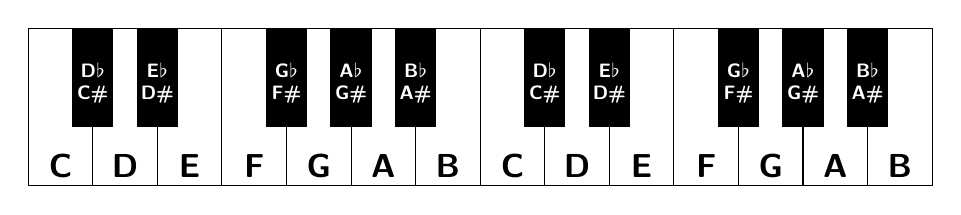
\begin{tikzpicture}[x=0.82cm,y=1cm,font=\sffamily\bfseries\scriptsize]
\foreach \n [count=\i from 0] in {C,D,E,F,G,A,B,C,D,E,F,G,A,B} {\draw (\i,0) rectangle (\i+1,2); \node at (\i+0.5,0.25) {\large\n};}
\foreach \x/\a/\b in {1/D/C,2/E/D,4/G/F,5/A/G,6/B/A,8/D/C,9/E/D,11/G/F,12/A/G,13/B/A}
  {\fill (\x-0.32,0.75) rectangle (\x+0.32,2); \node[white,align=center,inner sep=0pt] at (\x,1.3) {\a$\flat$\\\b\#};}
\end{tikzpicture}}\par\vspace{6pt}
\begin{gtable}{S No}{Quiz}{M}{BT}{CO}
\q{1.}{Construct the swara sequence for the 52\textsuperscript{nd} \ Melakartha (Ramapriya).}{2}{1}{2}
\q{2.}{Write the continued fraction expansion of $log_2(3/2)$ up to three terms.}{2}{2}{1}
\q{3.}{Give the Fourier series form of a periodic function and explain what the coefficients represent physically.}{2}{2}{2}
\q{4.}{Define the spectral centroid and compute it for a harmonic spectrum with amplitudes $A=\{5,3,1\}$ at frequencies $\{f, 2f, 3f\}$.}{2}{3}{3}
\q{5.}{Define a pitch class and express pitch class addition formally in modulo 12.}{2}{2}{3}
\end{gtable}
\par\vspace{8pt}
\begin{gtable}{S No}{Test}{M}{BT}{CO}
\q{1a}{Prove that $log_2(3/2)$ is irrational using proof by contradiction. Explain in detail the musical consequence of it.}{10}{2}{1}
\q{2a}{Derive the formula for (or explanation on) the total number of Melakartha rāgas (72) starting from the combinatorial possibilities of swaras, and elaborate on the \textit{Katapayadi sutra} therein.}{10}{3}{2}
\q{3}{Derive the mathematical explanation for difference tones using the nonlinear distortion equation: $y = ax + bx^2$. If two pure tones at frequencies f$_1$ and f$_2$ are input, show that the output contains the difference frequency $|f_1 - f_2|$.\newline
When two notes at 600 Hz and 800 Hz are played simultaneously:\newline
(i) Calculate the first-order difference tone.\newline
(ii) Calculate the first-order summation tone.\newline
(iii) Identify the musical interval represented by 600 Hz and 800 Hz.\newline
Also, explain why combination tones are more prominent in organs and brass instruments.}{10}{3}{4}
\q{4}{For a square wave $f(t)=\begin{cases}k\ for\ 0<t<\frac{T}{2}\\-k\ for\ \frac{T}{2}<t<T\end{cases}$, derive its Fourier series representation showing that it contains only odd harmonics with amplitudes decreasing as $1/n$. Explain why the square wave sounds different from a sawtooth wave despite both being periodic.}{\illegc}{\illegc}{\illegc}
\q{5}{Prove that the set of all transposition operations $\{T_0, T_1, T_2, \ldots, T_{11}\}$ forms a cyclic group under composition, isomorphic to $(\mathbb{Z}_{12}, +)$. Show that:\newline
(i) Closure: $T_m \circ T_n = T_{(m+n)}\ mod\ 12$\newline
(ii) Associativity holds\newline
(iii) Identity element exists\newline
(iv) Inverse elements exist}{\illegc}{\illegc}{\illegc}
\end{gtable}
\end{xpaper}

% ---------- EI375TGK Disease and Diagnostics an Engineering Perspective
\begin{iempaperB}
\paperinfo{ayear={2025-2026(ODDSem)},usn=0,dept={ELECTRONICS AND INSTRUMENTATION ENGINEERING},date={16.12.2025},code={EI375TGK},sem={VII},exam={CIE (Quiz \&Test) - 2},maxmarks={10+50},duration={120 Min},
 title={Course Title: DISEASE AND DIAGNOSTICS AN ENGINEERING PERSPECTIVE},shownote=0}
\iemheadB
\begin{gtable}{Sl.\newline No.}{PART-A}{M}{BT}{CO}
\q{1.1}{What is spirometry?}{1}{L1}{2}
\q{1.2}{Define Tidal Volume (TV) and Residual Volume (RV).}{2}{L1}{1}
\q{1.3}{What is Functional Residual Capacity (FRC)? Mention its components.}{2}{L2}{1}
\q{1.4}{Which lung capacity cannot be measured using spirometry?}{1}{L1}{1}
\q{1.5}{Name two types of dialysis.}{1}{L1}{2}
\q{1.6}{Define kidney filtration.}{1}{L1}{3}
\q{1.7}{What is a dialyzer?}{1}{L1}{3}
\q{1.8}{What is creatinine?}{1}{L1}{3}
\end{gtable}
\btfoot{|l|l|l|*{10}{C{0.8cm}|}}{\hline
\multirow{2}{*}{\shortstack{Marks\\Distribution}} & \multicolumn{2}{c|}{Particulars} & CO1 & CO2 & CO3 & CO4 & L1 & L2 & L3 & L4 & L5 & L6\\\cline{2-13}
 & Test & \shortstack{Max\\Marks} & 05 & 02 & 03 & - & 8 & 2 & - & - & - & -\\\hline}
\stars{***********}
\par\vspace{6pt}
\begin{gtable}{Sl.\newline No.}{PART- B}{M}{BT}{CO}
\q{1.}{Explain the functioning of the Respiratory System (RS).}{10}{L1}{1}
\q{2.}{Explain lung volumes and capacities with a neatly labeled diagram.}{10}{L2}{2}
\q{3.}{Describe any four common diseases of the Renal System.}{10}{L1}{3}
\q{4.}{Explain the structure and functioning of the Renal System.}{10}{L2}{1}
\q{5.}{Describe common ailments of the respiratory system, their causes, and symptoms.}{10}{L2}{3}
\end{gtable}
\btfoot{|l|l|l|*{10}{C{0.8cm}|}}{\hline
\multirow{2}{*}{\shortstack{Marks\\Distribution}} & \multicolumn{2}{c|}{Particulars} & CO1 & CO2 & CO3 & CO4 & L1 & L2 & L3 & L4 & L5 & L6\\\cline{2-13}
 & Test & \shortstack{Max\\Marks} & 20 & 10 & 20 & - & 20 & 30 & - & - & - & -\\\hline}
\stars{***********}
\end{iempaperB}

% ---------- Indian Knowledge System: a second Part-B (Test) page; its header and Part A are not in the scanned copy
\begin{xpaper}
\par\vspace{2pt}\centerline{\small\itshape [Indian Knowledge System -- a second CIE-II test page. The header and Part A of this paper are not in the scanned copy.]}\par\vspace{8pt}
\begin{longtable}{|C{1.05cm}|p{13.15cm}|C{0.95cm}|C{0.95cm}|}
\multicolumn{4}{c}{\bfseries TEST}\\*[2pt]
\hline \textbf{Sl.\newline No.} & \multicolumn{1}{c|}{\textbf{Part- B Questions}} & \textbf{M} & \illegc\\* \hline
1 a & List the six classical schools of Indian philosophy. & 03 & \multirow{4}{*}{\illegc}\\*
b & Explain any two threats to traditional knowledge. & 02 & \\*
c & Mention one key difference between traditional Indian and Western systems of knowledge. & 02 & \\*
d & How does the Vedic Corpus form the foundation of Indian knowledge traditions? & 03 & \\\hline
2 a & Draw a neat framework for classification of IKS Corpus & 03 & \multirow{4}{*}{\illegc}\\*
b & Name the six Vedangas. & 03 & \\*
c & State the two types of perception recognized in Nyaya philosophy & 02 & \\*
d & Differentiate between agricultural and ecological traditional knowledge. & 02 & \\\hline
3 a & Mention any four Yogasutra of Patanjali & 03 & \multirow{4}{*}{1}\\*
b & Describe the characteristics and scope of Indian traditional knowledge in the modern context. & 03 & \\*
c & Mention one key feature that differentiates Nyaya from Samkhya philosophy. & 02 & \\*
d & Name the six orthodox (\textit{āstika}) schools of Indian philosophy & 02 & \\\hline
4 a & Find out the difference from the Kaṭapayādi system to Bhūta-saṅkhyā for the word ``Rāma''. & 03 & \multirow{4}{*}{2}\\*
b & Name the three generic measures used in the ancient Indian system. & 02 & \\*
c & Laghu and Guru syllables in the given word: {\fontspec[Script=Devanagari]{Nirmala UI}योगदर्शन} (yōgadarśana) & 02 & \\*
d & Develop a binary cycle of length four and identify all possible binary words of length fours. & 03 & \\\hline
5 a & What is the standardized units for street widths in Indus-Saraswati civilization? & 02 & \multirow{4}{*}{3}\\*
b & Who the concept \ of zero discovered in India? What is its special significance? & 03 & \\*
c & What is the numeral representation for the word `manu, agni, elephant, Tithi, rudra, Indra, Pandava. & 03 & \\*
d & Briefly provide the organization of ``Ashtadhyayi''. How many rules are there in Ashtadhyayi ? & 02 & \\\hline
\end{longtable}
\par\vspace{2pt}\centerline{\small\itshape [The heading of the fourth column and the column after it are cut off in the scan.]}
\btfoot{|l|l|l|*{10}{C{0.8cm}|}}{\hline
\multirow{2}{*}{\shortstack{Marks\\Distribution}} & \multicolumn{2}{c|}{Particulars} & CO1 & CO2 & CO3 & CO4 & L1 & L2 & L3 & L4 & L5 & L6\\\cline{2-13}
 & Test & \shortstack{Max\\Marks} & 10 & 10 & 5 & --- & 15 & 10 & --- & --- & --- & ---\\\hline}
\end{xpaper}

\end{document}
